%% myFigures.tex
% A common file to store all figure definitions
%
% In preparing your thesis, one of the first things you should do is
% organize your figures.  Then, one of the last things you'll do is
% reorder your figures so they display where you want them to in the
% text.  Organizing figure definitions in a common files helps:
%
%   1. Write new figures using earlier examples.
%
%   2.  Isolate code and minimize the risk of introducing bugs in the
%   final editing process.  Trust me, moving around just one line of
%   code is easier.
%
%   3.  Reuse figures in other papers.  <=== the best reason!
%
% Note command names can not include numbers and special characters.
%
% To make the file more searchable, use naming conventions that map
% the graphics filename labSetup.jpg to the command name \figlabSetup to the
% figure label fig:labSetup.
% 

\newcommand{\figproactiveFaultManagement}[1]{\begin{figure}[H]
 \begin{center}
    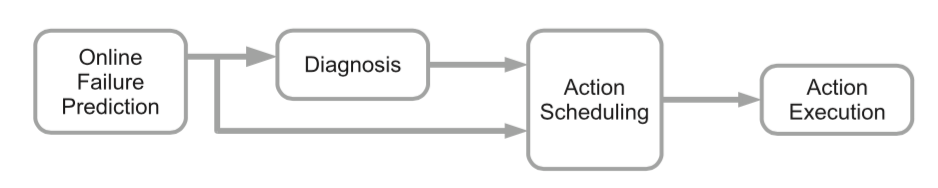
\includegraphics[width=#1]{proactiveFaultManagement}
     \caption[Proactive Fault Management~\cite{salfnerSurvey}]{The stages of
     proactive fault management~\cite{salfnerSurvey}.}
     \label{fig:proactiveFaultManagement}
 \end{center}
\end{figure}
}

\newcommand{\figonlinePrediction}[1]{\begin{figure}[H]
 \begin{center}
    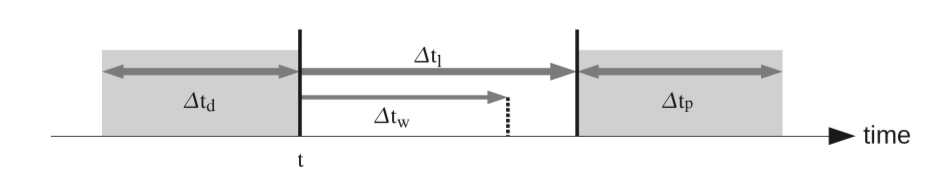
\includegraphics[width=#1]{onlinePrediction}
     \caption[Online Failure Prediction~\cite{salfnerSurvey}]{The timeline for
     OFP~\cite{salfnerSurvey}.}
     \label{fig:onlinePrediction}
 \end{center}
\end{figure}
}

\newcommand{\figfailureFlowDiagram}[1]{\begin{figure}[H]
 \begin{center}
    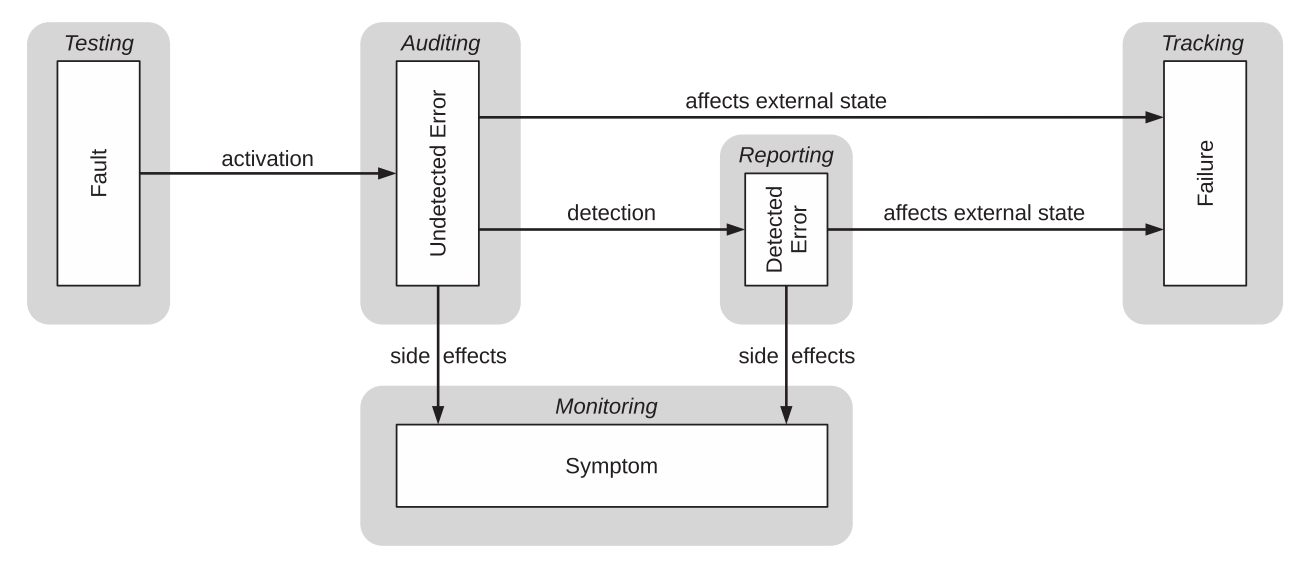
\includegraphics[width=#1]{failureFlowDiagram}
     \caption[Failure Flow Diagram~\cite{salfnerSurvey}]{How faults and errors
     evolve into failure with the associated methods for detection represented
     by enclosing gray boxes~\cite{salfnerSurvey}.}
     \label{fig:failureFlowDiagram}
 \end{center}
 %\vspace{-0.2 in}
\end{figure}
}

\newcommand{\figROC}[1]{\begin{figure}[H]
 \begin{center}
    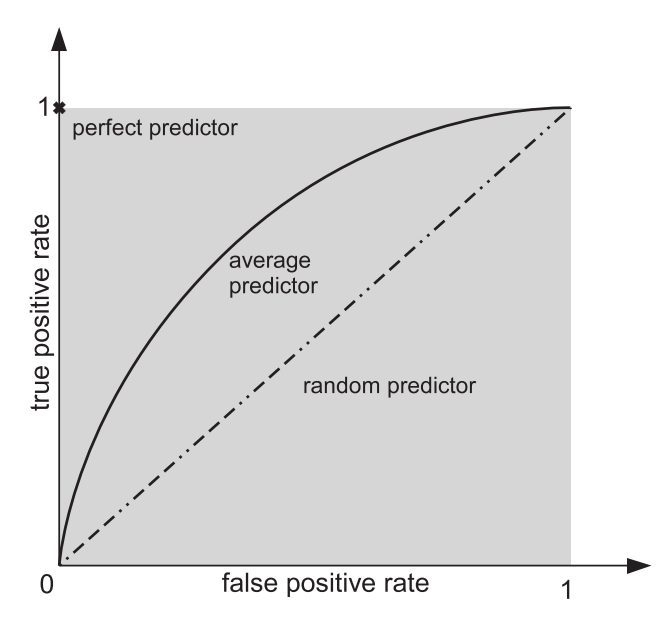
\includegraphics[width=#1]{ROC}
     \caption[Sample ROC Plots~\cite{salfnerSurvey}]{ROC plots of perfect,
     average, and random predictors~\cite{salfnerSurvey}.}
     \label{fig:ROC}
 \end{center}
\end{figure}
}

\newcommand{\figprecisionRecallCurve}[1]{\begin{figure}[H]
 \begin{center}
    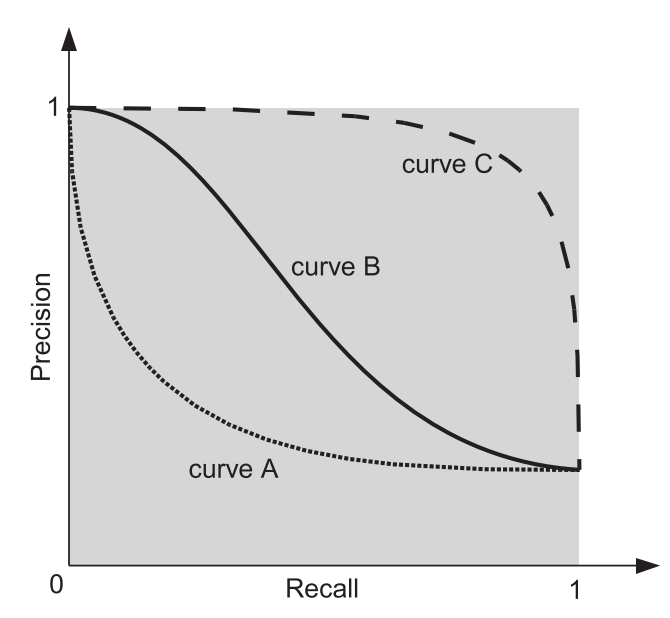
\includegraphics[width=#1]{precisionRecallCurve}
     \caption[Sample Precision/Recall Curves~\cite{salfnerSurvey}]{Sample
     precision/recall curves~\cite{salfnerSurvey}.  Curve $A$ represents a
     poorly performing predictor, curve $B$ an average predictor, and curve $C$
     an exceptional predictor.}
     \label{fig:precisionRecallCurve}
 \end{center}
\end{figure}
}

\newcommand{\figpatternRecognition}[1]{\begin{figure}[H]
 \begin{center}
    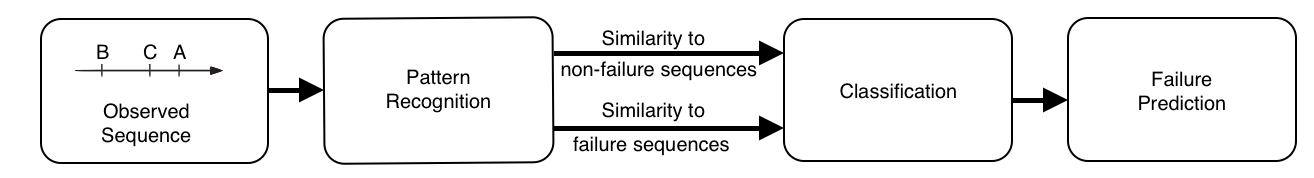
\includegraphics[width=#1]{patternRecognition}
     \caption[Pattern recognition in reported errors~\cite{salfnerSurvey}]{How
     pattern recognition is accomplished in reported
     errors~\cite{salfnerSurvey}.}
     \label{fig:patternRecognition}
 \end{center}
\end{figure}
}

\newcommand{\figAFP}[1]{\begin{figure}[H]
 \begin{center}
    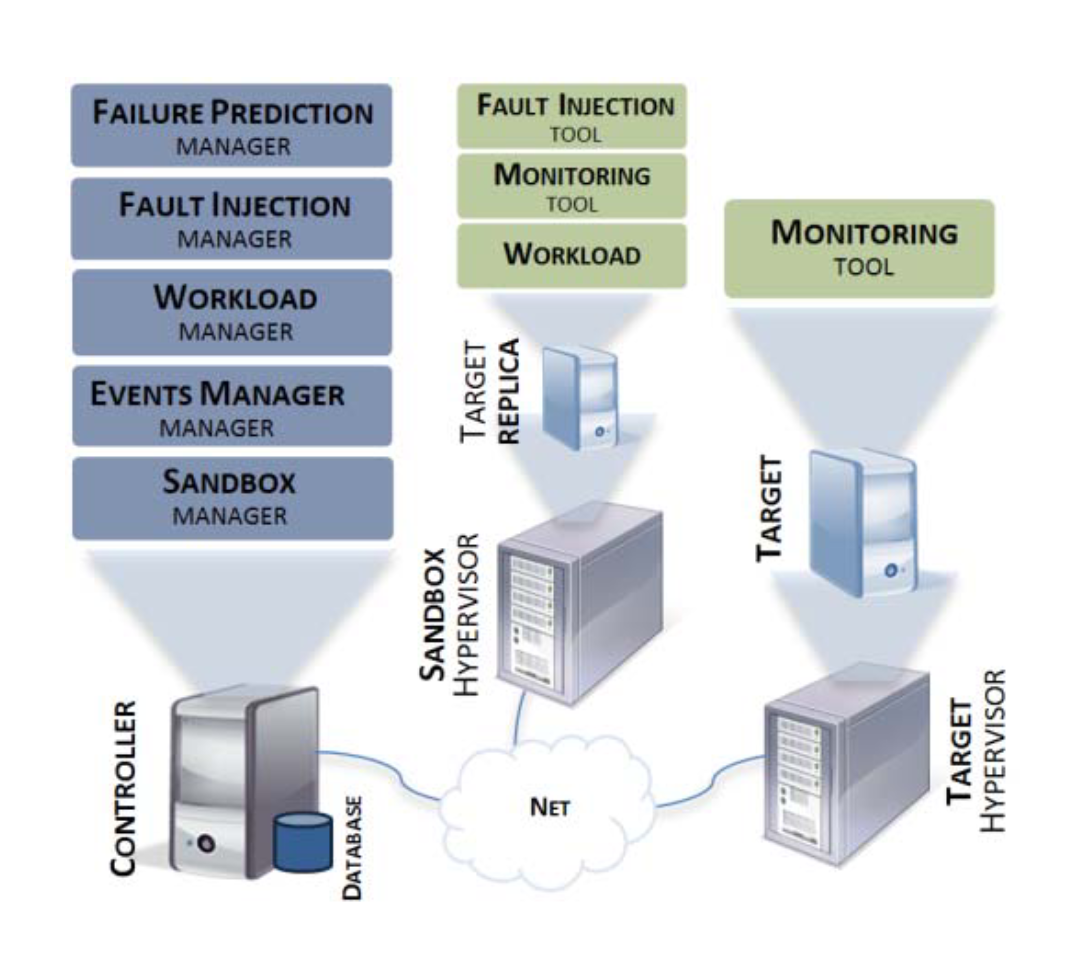
\includegraphics[width=#1]{AFP}
     \caption[AFP Framework Implementation~\cite{irrera2015}]{How the AFP
     framework is implemented~\cite{irrera2015}.}
     \label{fig:AFP}
 \end{center}
\end{figure}
}

\definecolor{airforceblue}{rgb}{0.36, 0.54, 0.66}
\definecolor{armygreen}{rgb}{0.29, 0.33, 0.13}

\newcommand{\figannotatedAFPcolor}{\begin{figure}[ht!]
 \begin{center}
     \begin{overpic}[width=5in,scale=.25]{annotatedAFPcolor}
       \put(8,0){
         \begin{tikzpicture}
           [node font=\footnotesize, label/.style={rectangle, draw,
           fill=airforceblue, text width=2cm, text badly centered, minimum
           height=0.5cm, rounded corners}]

           \node[label] (FPMgr)
             {\textcolor{white}{\ref{sec:failurePrediction}}};
           \node[label, below=1.2cm of FPMgr] (FIMgr) 
             {\textcolor{white}{\ref{sec:faultInjectionMgr}}};
           \node[label, below=1.3cm of FIMgr] (WMgr) 
             {\textcolor{white}{\ref{sec:workloadMgr}}};
           \node[label, below=1.2cm of WMgr] (EMMgr) 
             {\textcolor{white}{\ref{sec:eventsManagerMgr}}};
           \node[label, below=1.2cm of EMMgr] (SMgr) 
             {\textcolor{white}{\ref{sec:sandboxMgr}}};
           \node[label, below=4.75cm of SMgr] (Controller) 
             {\textcolor{white}{\ref{sec:controller}}};
         \end{tikzpicture}
       }

       \put(40,60.5){
         \begin{tikzpicture}
           [node font=\footnotesize, label/.style={rectangle, draw,
           fill=armygreen, text width=2cm, text badly centered, minimum
           height=0.5cm, rounded corners}]

           \node[label] (Sandbox)
             {\textcolor{white}{\ref{sec:sandbox}}};
           \node[label, below=1.2cm of Sandbox] (SBFITool)
             {\textcolor{white}{\ref{sec:faultInjectionTool}}};
           \node[label, below=0.95cm of SBFITool] (SBMTool) 
             {\textcolor{white}{\ref{sec:sandboxMonitoringTool}}};
           \node[label, below=0.95cm of SBMTool] (SBWorkload) 
             {\textcolor{white}{\ref{sec:sandboxWorkload}}};
         \end{tikzpicture}
       }

       \put(66,0){
         \begin{tikzpicture}
           [node font=\footnotesize, label/.style={rectangle, draw,
           fill=armygreen, text width=2cm, text badly centered, minimum
           height=0.5cm, rounded corners}]

           \node[label] (MonTool)
             {\textcolor{white}{\ref{sec:targetMonitoringTool}}};
           \node[label, below=7.85cm of MonTool] (Target)
             {\textcolor{white}{\ref{sec:target}}};
         \end{tikzpicture}
       }
     \end{overpic}
     \caption[Annotated AFP Framework~\cite{irrera2015}]{The AFP framework
     implementation~\cite{irrera2015} with modified components highlighted.}
     \label{fig:annotatedAFP}
 \end{center}
\end{figure}
}

\newcommand{\figannotatedAFP}{\begin{figure}[ht!]
 \begin{center}
     \begin{overpic}[width=5in,scale=.25]{annotatedAFP}
       \put(8,0){
         \begin{tikzpicture}
           [node font=\footnotesize, label/.style={rectangle, draw,
           fill=white, text width=2cm, text badly centered, minimum
           height=0.5cm, rounded corners}]

           \node[label] (FPMgr)
             {\textcolor{black}{\ref{sec:failurePrediction}}};
           \node[label, below=1.2cm of FPMgr] (FIMgr) 
             {\textcolor{black}{\ref{sec:faultInjectionMgr}}};
           \node[label, below=1.3cm of FIMgr] (WMgr) 
             {\textcolor{black}{\ref{sec:workloadMgr}}};
           \node[label, below=1.2cm of WMgr] (EMMgr) 
             {\textcolor{black}{\ref{sec:eventsManagerMgr}}};
           \node[label, below=1.2cm of EMMgr] (SMgr) 
             {\textcolor{black}{\ref{sec:sandboxMgr}}};
           \node[label, below=4.75cm of SMgr] (Controller) 
             {\textcolor{black}{\ref{sec:controller}}};
         \end{tikzpicture}
       }

       \put(40,60.5){
         \begin{tikzpicture}
           [node font=\footnotesize, label/.style={rectangle, draw,
           fill=white, text width=2cm, text badly centered, minimum
           height=0.5cm, rounded corners}]

           \node[label] (Sandbox)
             {\textcolor{black}{\ref{sec:sandbox}}};
           \node[label, below=1.2cm of Sandbox] (SBFITool)
             {\textcolor{black}{\ref{sec:faultInjectionTool}}};
           \node[label, below=0.95cm of SBFITool] (SBMTool) 
             {\textcolor{black}{\ref{sec:sandboxMonitoringTool}}};
           \node[label, below=0.95cm of SBMTool] (SBWorkload) 
             {\textcolor{black}{\ref{sec:sandboxWorkload}}};
         \end{tikzpicture}
       }

       \put(66,0){
         \begin{tikzpicture}
           [node font=\footnotesize, label/.style={rectangle, draw,
           fill=white, text width=2cm, text badly centered, minimum
           height=0.5cm, rounded corners}]

           \node[label] (MonTool)
             {\textcolor{black}{\ref{sec:targetMonitoringTool}}};
           \node[label, below=7.85cm of MonTool] (Target)
             {\textcolor{black}{\ref{sec:target}}};
         \end{tikzpicture}
       }
     \end{overpic}
     \caption[Annotated AFP Framework~\cite{irrera2015}]{The AFP framework
     implementation~\cite{irrera2015} with modified components highlighted.}
     \label{fig:annotatedAFP}
 \end{center}
\end{figure}
}

\newcommand{\figTrainingPhase}[1]{\begin{figure}[H]
 \begin{center}
  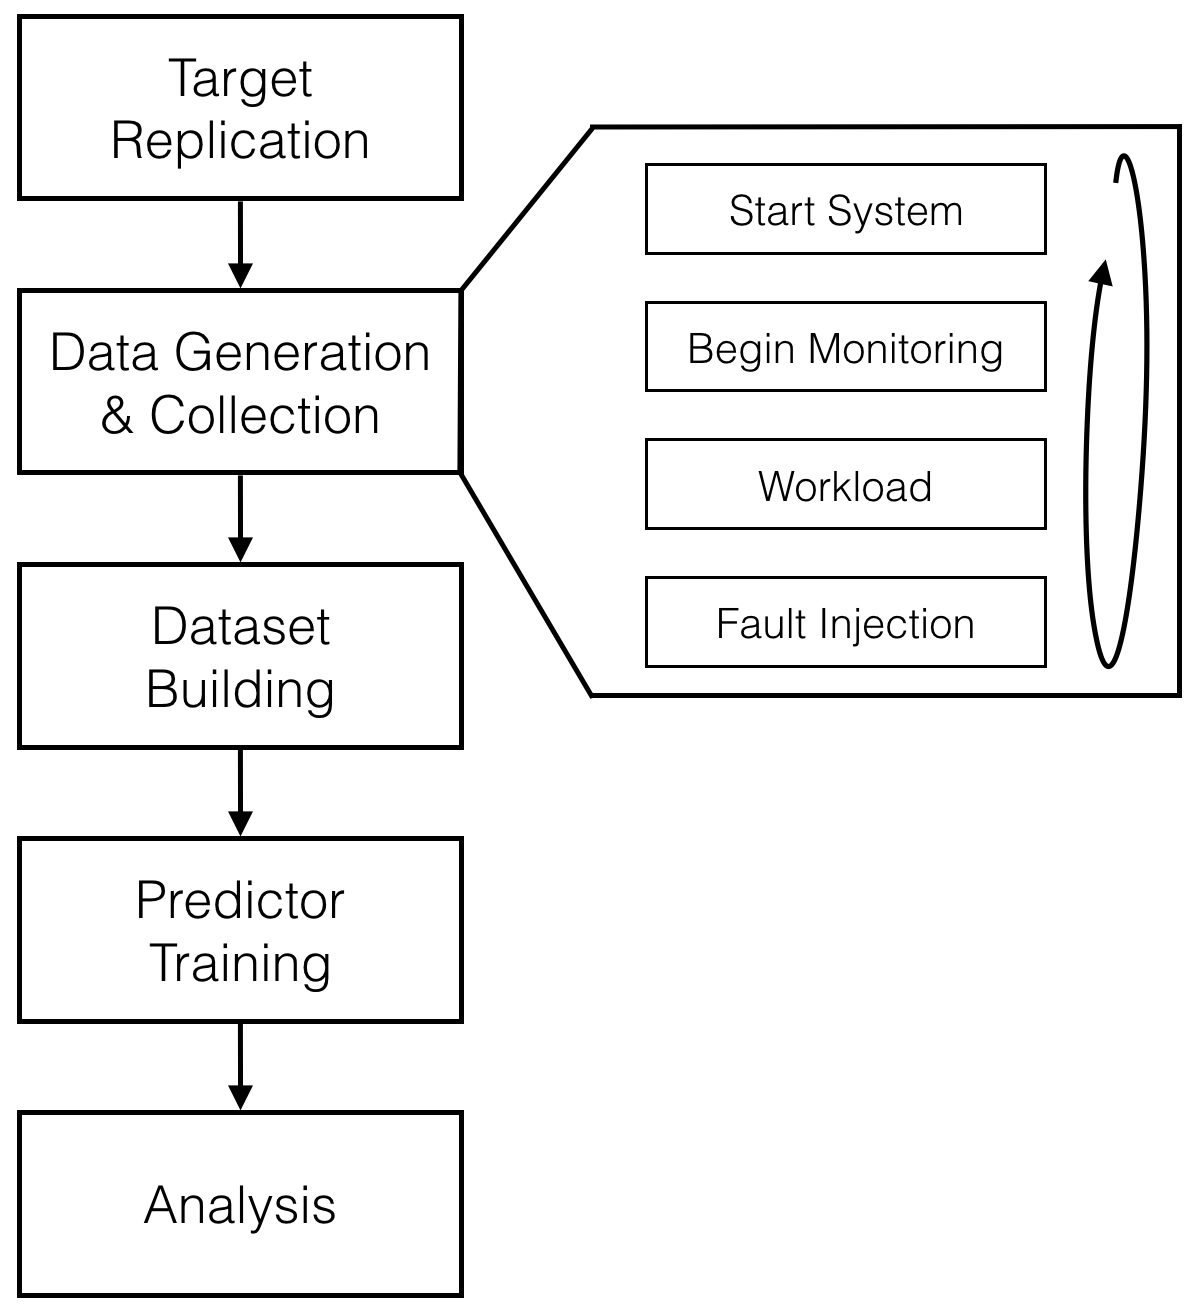
\includegraphics[width=#1]{TrainingPhase}
  \caption[AFP Training Phase~\cite{irrera2015}]{The flow of the major steps
    involved in the AFP framework training phase~\cite{irrera2015}.}
  \label{fig:TrainingPhase}
 \end{center}
\end{figure}
}

\newcommand{\figExecutionPhase}[1]{\begin{figure}[!ht]
  \begin{center}
    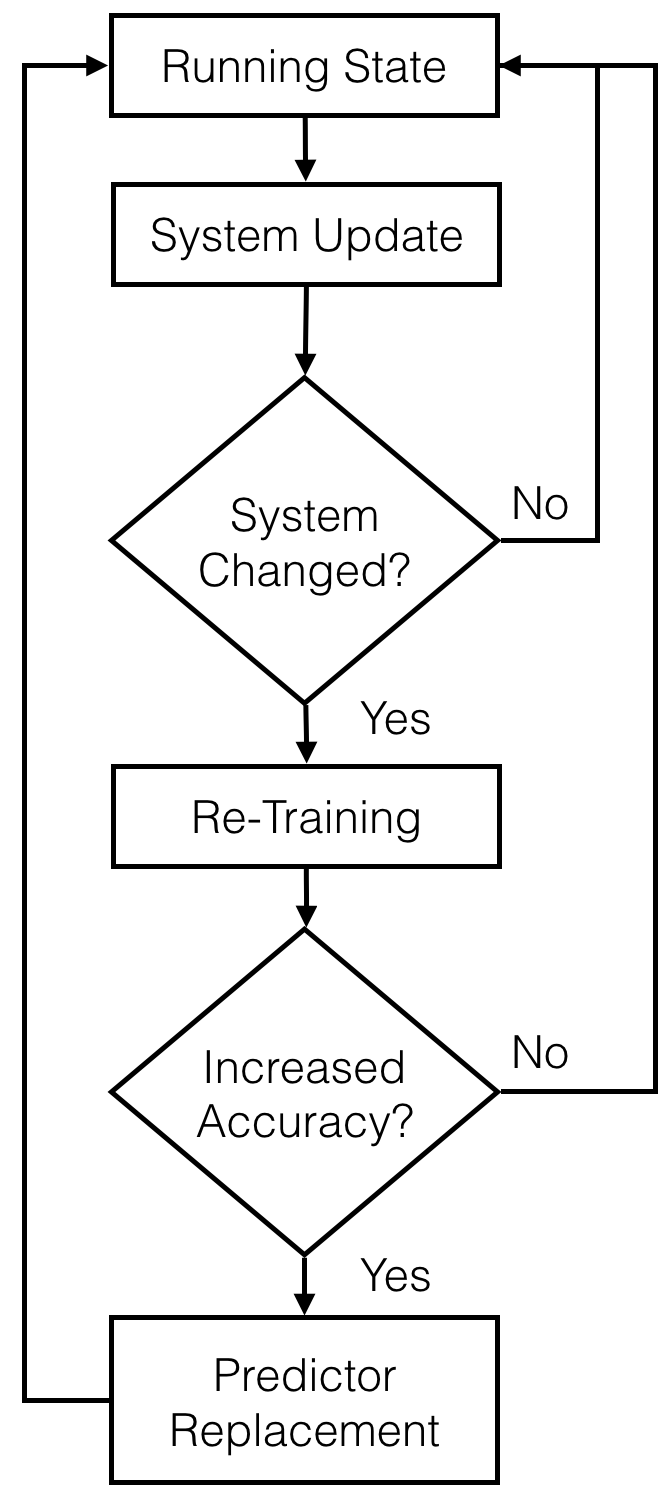
\includegraphics[width=#1]{ExecutionPhase}
    \caption[AFP Execution Phase~\cite{irrera2015}]{The flow of the major steps
    involved in the AFP framework execution phase~\cite{irrera2015}.}
    \label{fig:ExecutionPhase}
  \end{center}
\end{figure}
}

\newcommand{\figAuthDCPPS}[1]{\begin{figure}[ht!]
 \begin{center}
  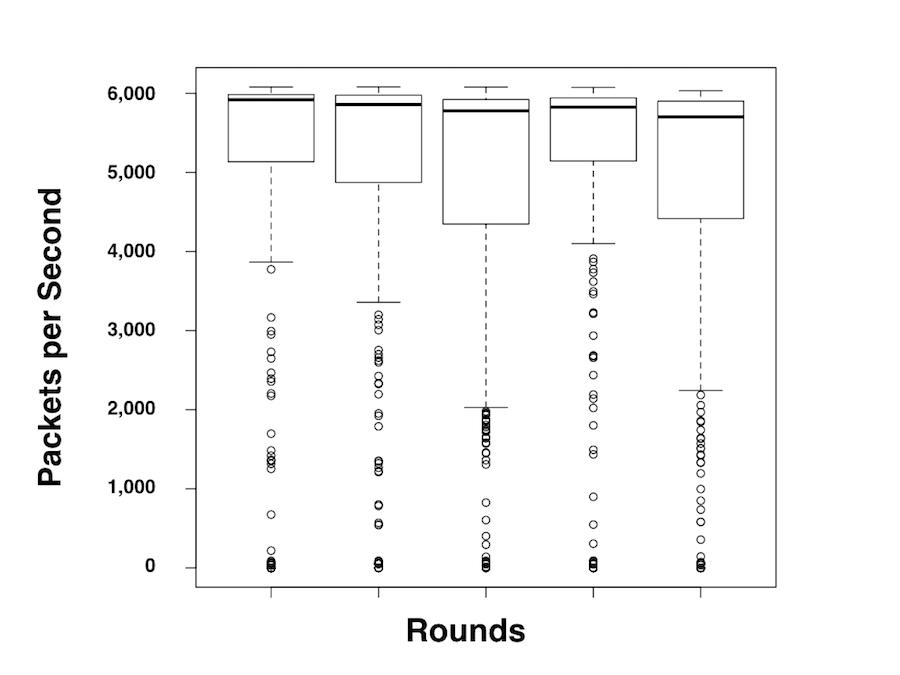
\includegraphics[width=#1]{authDCPPS}
  \caption[Domain Controller Packets per Second]{How many packets per second
  were sent or received by the domain controller across all five rounds of the
  first test.  In each test, we captured approximately 1.8 million packets.}
  \label{fig:authDCPPS}
 \end{center}
\end{figure}
}

\newcommand{\figAuthClientPPS}[1]{\begin{figure}[ht!]
 \begin{center}
  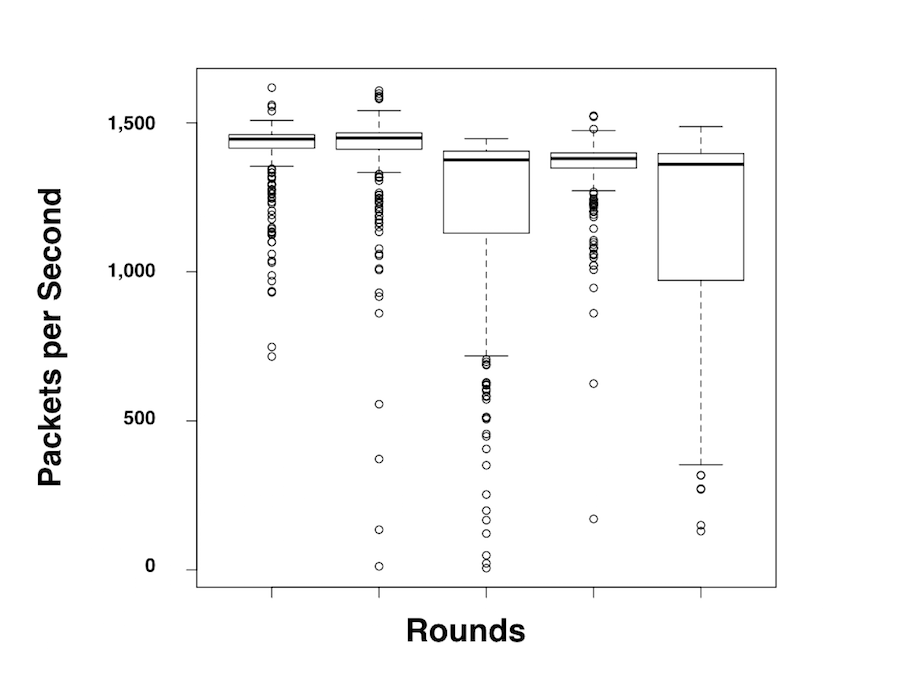
\includegraphics[width=#1]{authClientPPS}
  \caption[Client Packets per Second]{How many packets per second were sent or
  received by one of the clients across all five rounds of the first test.}
  \label{fig:authClientPPS}
 \end{center}
\end{figure}
}

\newcommand{\figAuthDCMetrics}[1]{\begin{figure}[ht!]
 \begin{center}
  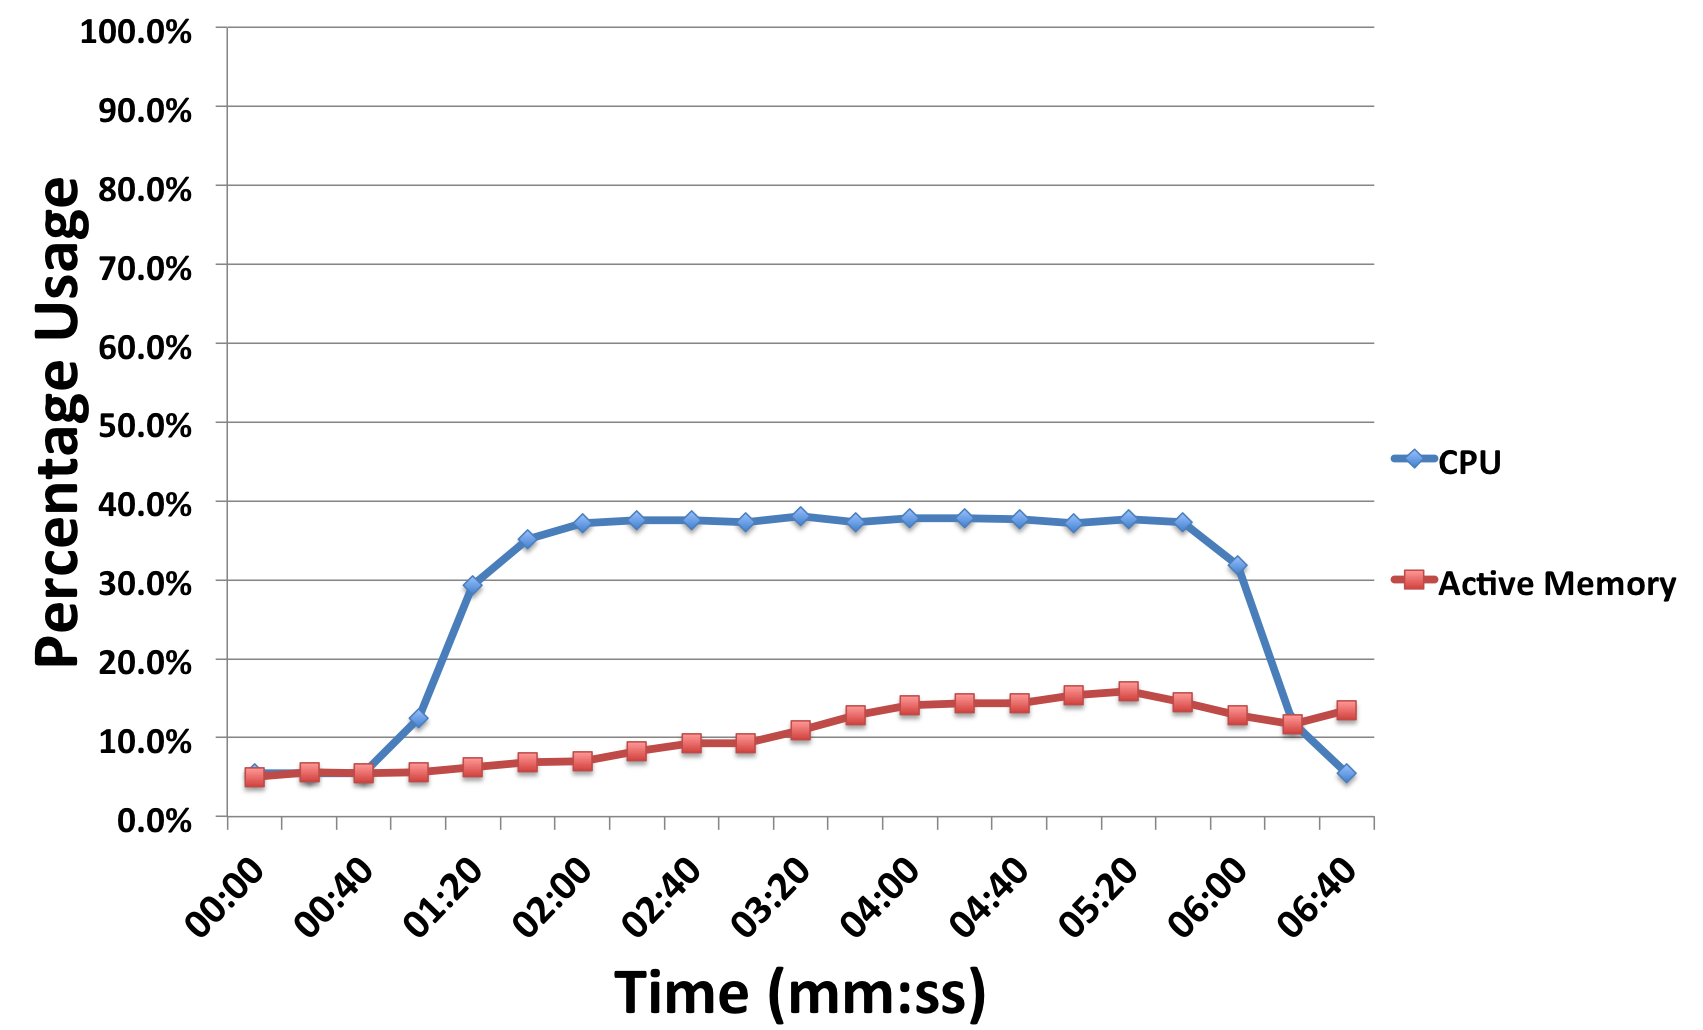
\includegraphics[width=#1]{authDCMetrics}
  \caption[Test 1:  Domain Controller Performance]{Domain controller CPU and
  memory utilization during the first test.}
  \label{fig:authDCMetrics}
 \end{center}
\end{figure}
}

\newcommand{\figOFPTaxonomy}[1]{\begin{figure}[ht!]
 \begin{center}
  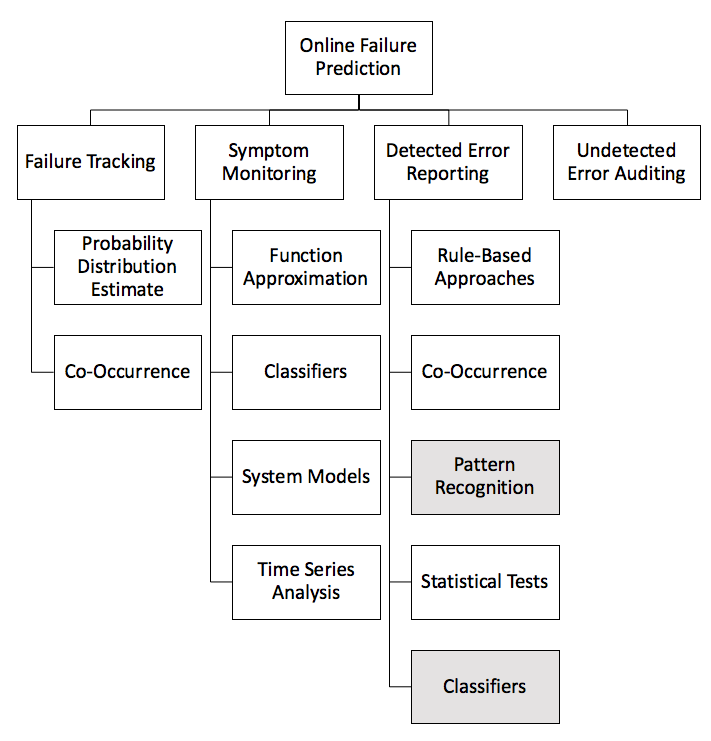
\includegraphics[width=#1]{OFPTaxonomy}
  \caption[Taxonomy of OFP Approaches]{Taxonomy of approaches to online
  failure prediction~\cite{salfnerSurvey}.  The two categories into which this
  research falls are highlighted.}
  \label{fig:OFPTaxonomy}
 \end{center}
\end{figure}
}

\newcommand{\figMemLeakROC}[1]{\begin{figure}[ht!]
 \begin{center}
  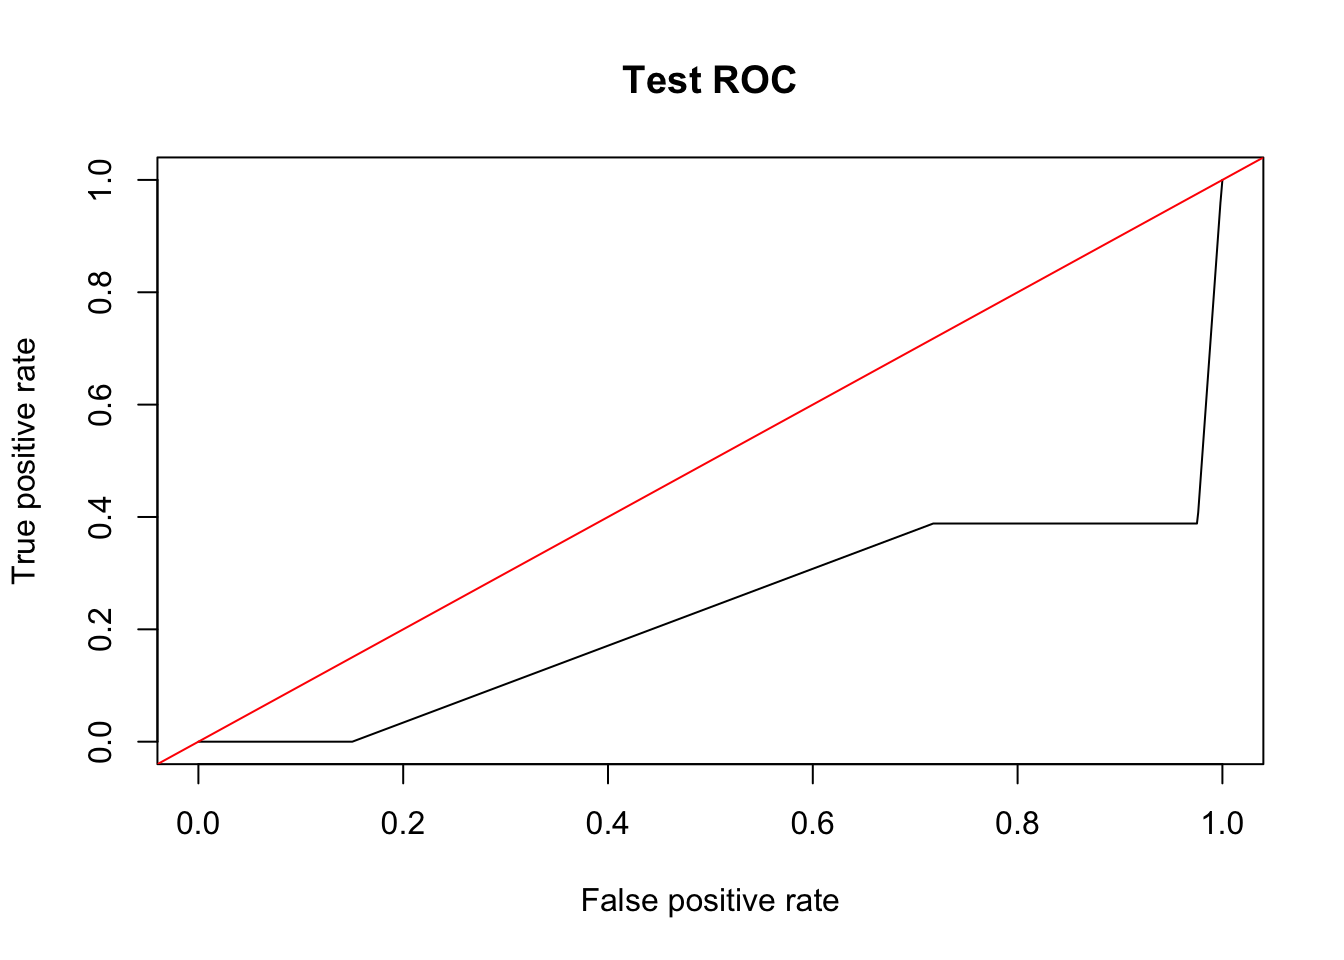
\includegraphics[width=#1]{MemLeakROC}
  \caption[SVM Memory Leak ROC Curve]{SVM memory leak test data ROC curve.}
  \label{fig:memLeakROC}
 \end{center}
\end{figure}
}

\newcommand{\figMemLeakCompare}[1]{\begin{figure}[ht!]
 \begin{center}
  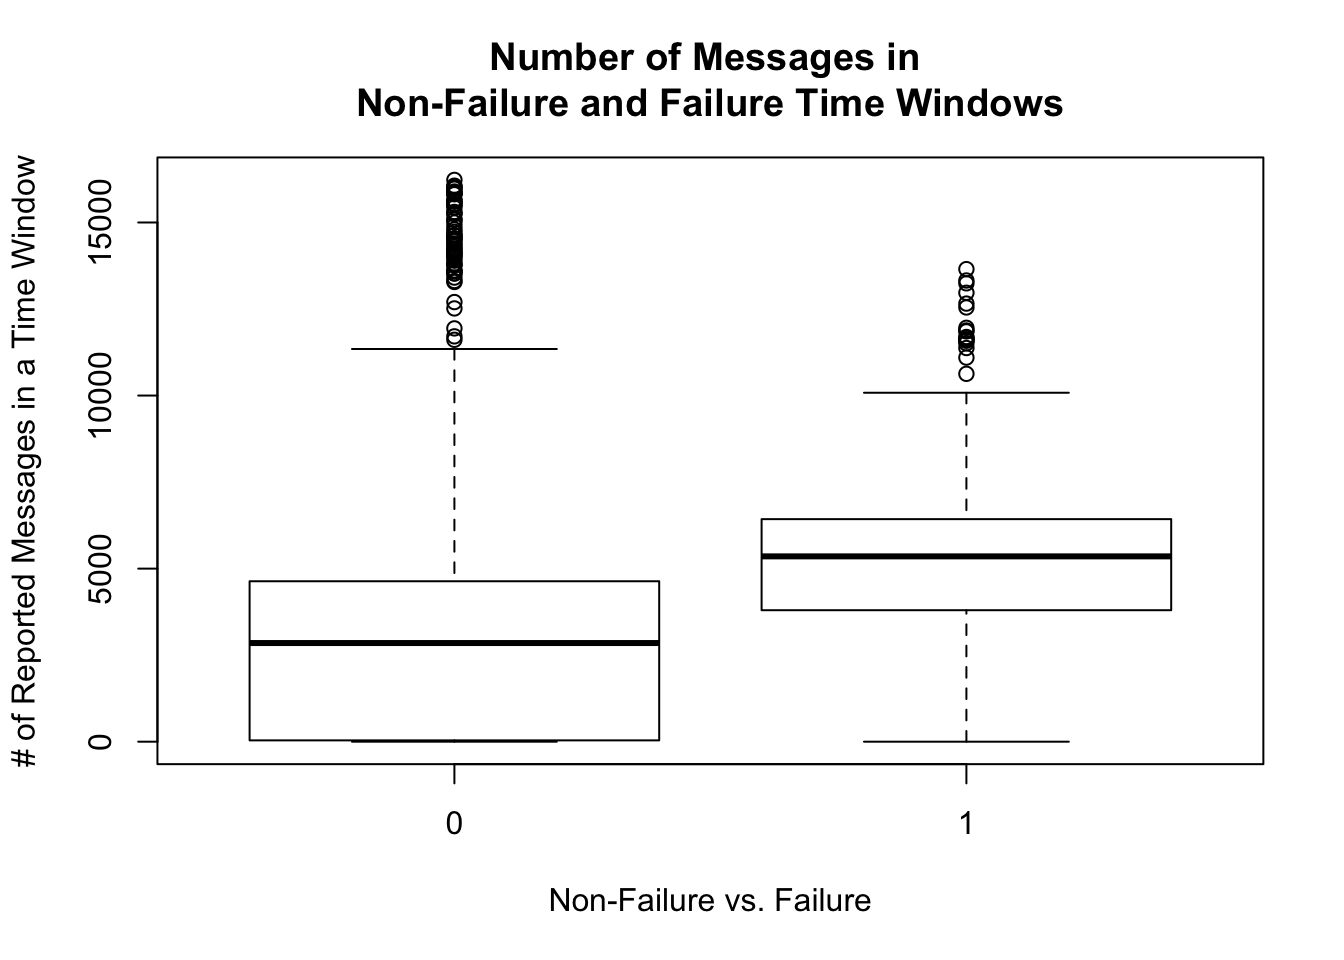
\includegraphics[width=#1]{MemLeakCompare}
  \caption[SVM Memory Leak Performance Comparison]{Number of observations in a
  given thirty second time window where `1' represents a window during which
  failure occurred and `0' represents a window during which no failure
  occurred.}
  \label{fig:memLeakCompare}
 \end{center}
\end{figure}
}

%%%%   SMV   %%%%
% Pre-Update
\newcommand{\figMemLeakPreUpdateSVMPerf}{\begin{figure*}[ht!]
  \centering
  \subfigure[Precision/Recall Curve.]{
    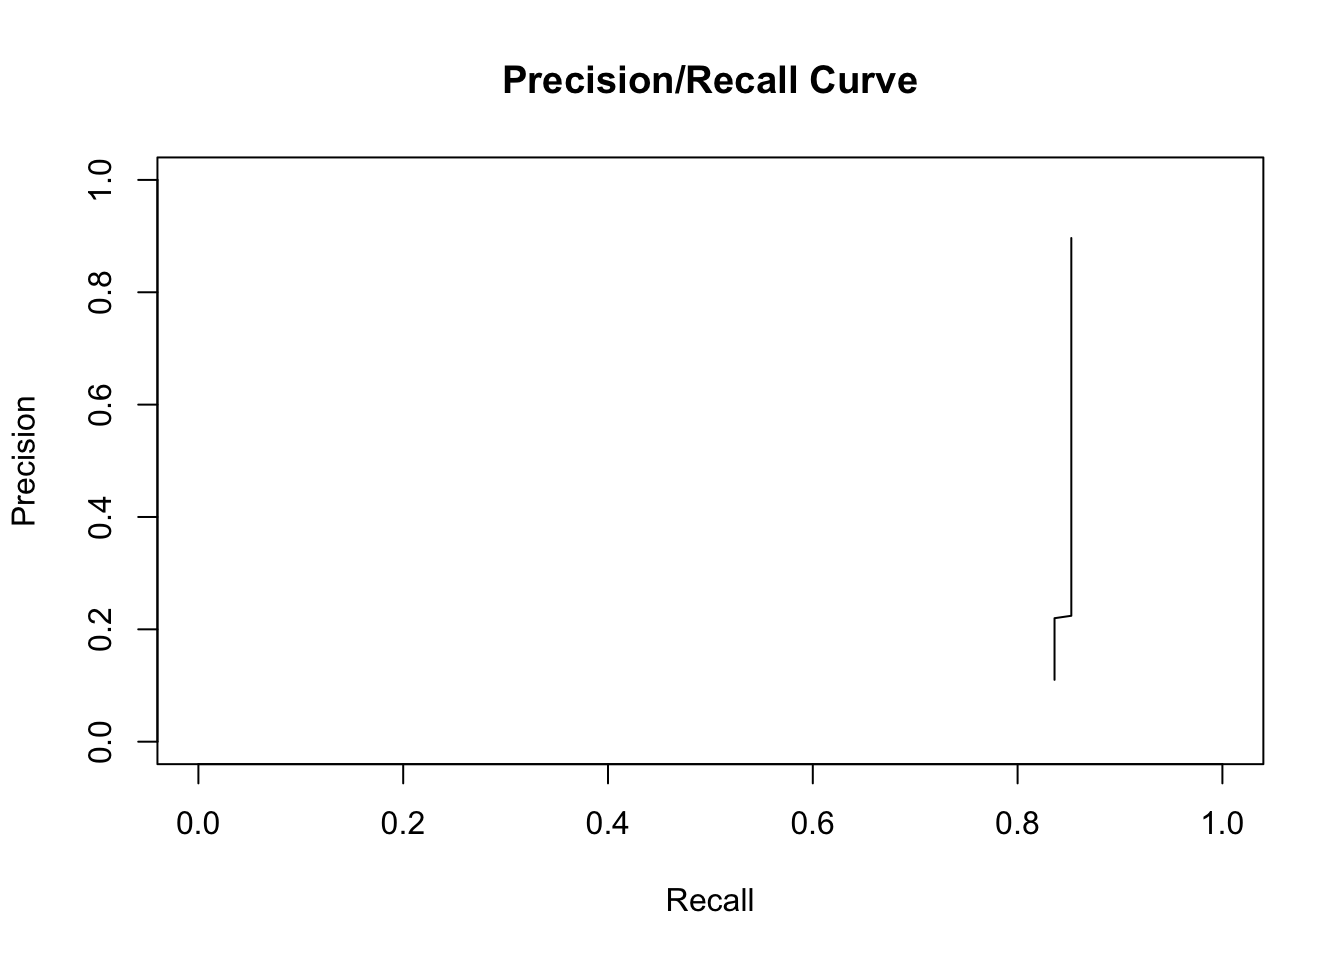
\includegraphics[width=0.45\textwidth]{results/pre-update/memleak/svm-prc}
  }
  \subfigure[Receiver Operating Characteristic (ROC) Curve (AUC = 0.8664).]{
    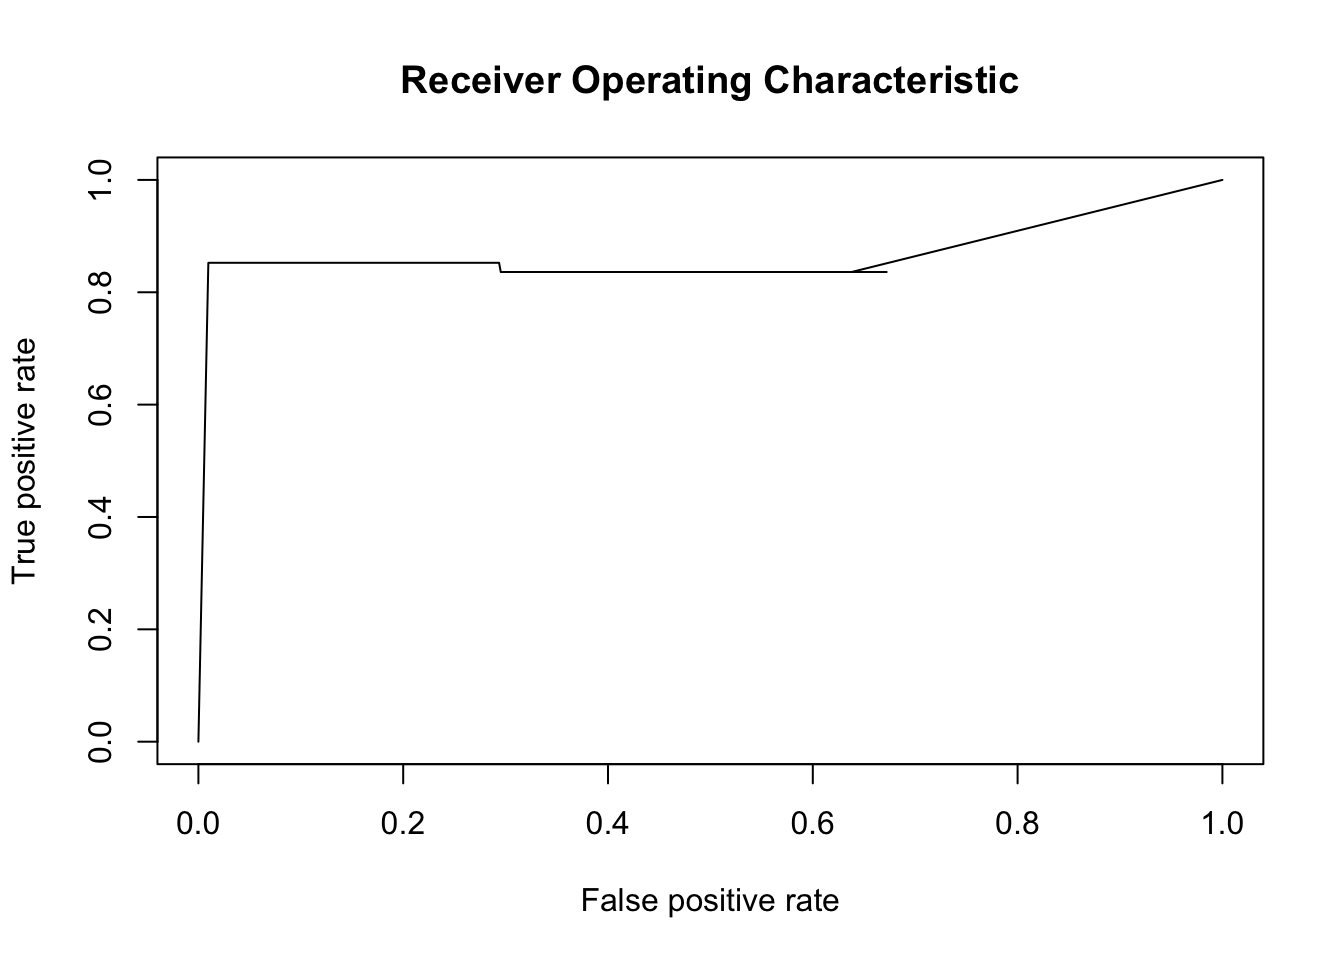
\includegraphics[width=0.45\textwidth]{results/pre-update/memleak/svm-roc}
  }
  \caption[Pre-Update, Memory Leak SVM Performance]{Test data performance of
  the SVM prediction method on failure data obtained by consuming all available
  memory until target application fails.} \label{fig:memLeakPreUpdateSVMPerf}
\end{figure*}
}

% Post-Update (old model)

% Post-Update New Model

%%%%   BOOSTING   %%%%
% Pre-Update
\newcommand{\figMemLeakPreUpdateBoostingPerf}{\begin{figure*}[ht!]
  \centering
  \subfigure[Precision/Recall Curve.]{
    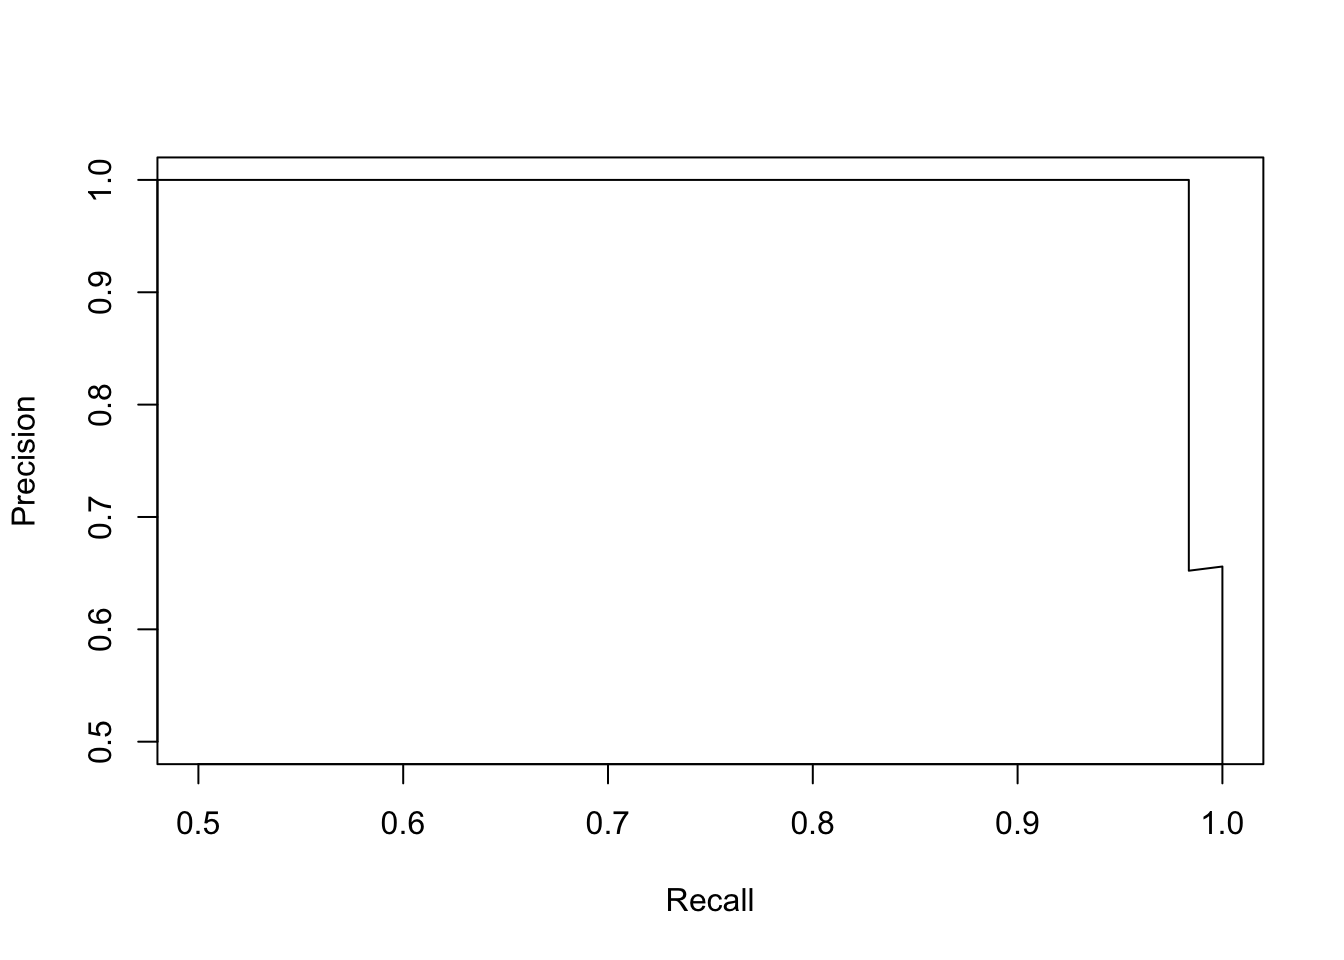
\includegraphics[width=0.45\textwidth]{results/pre-update/memleak/boosting-prc}
  }
  \subfigure[Receiver Operating Characteristic (ROC) Curve (AUC = 0.9984).]{
    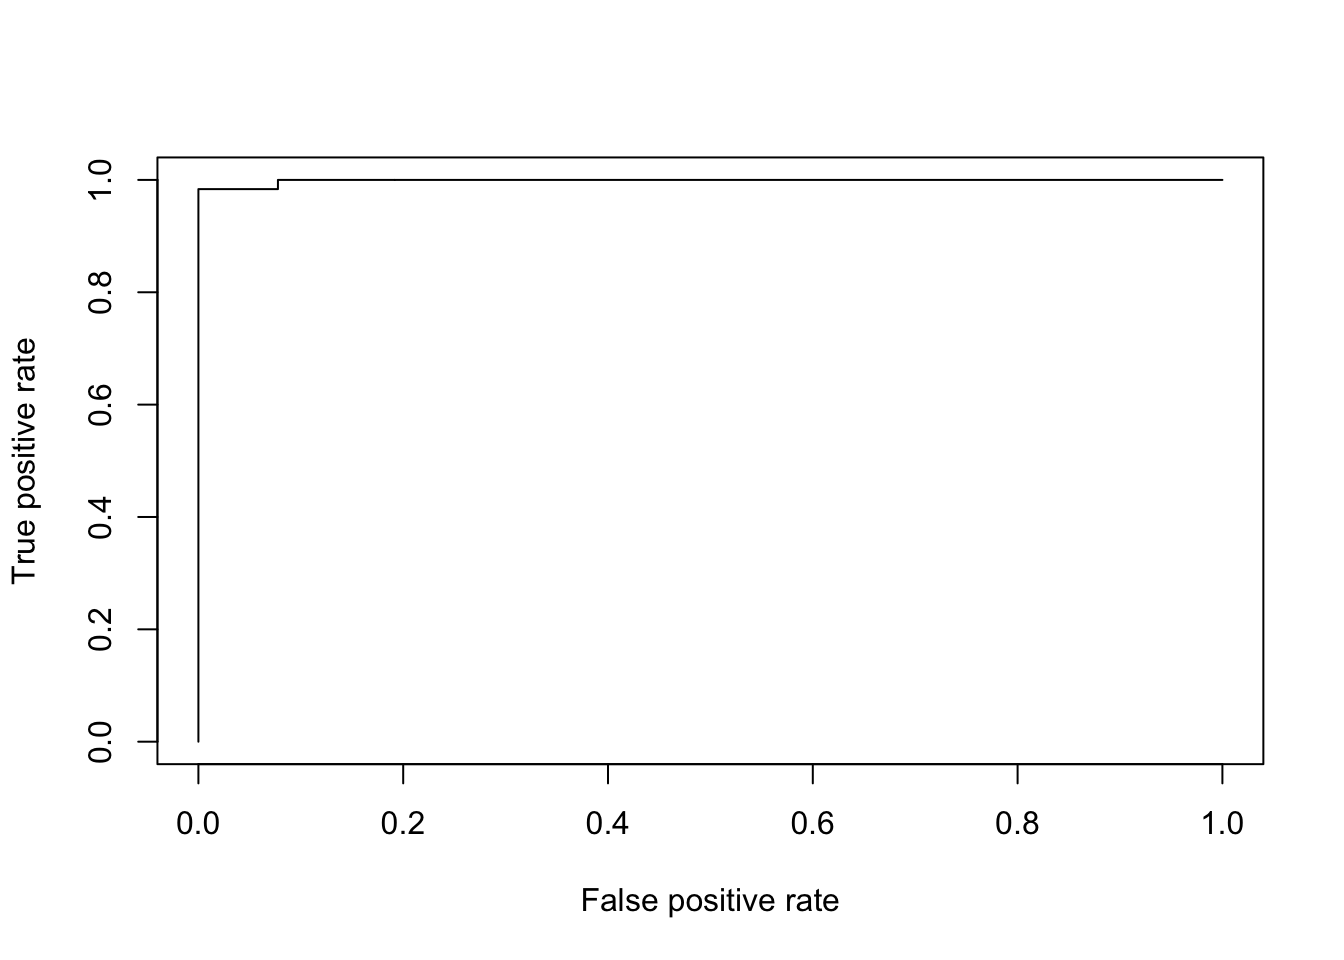
\includegraphics[width=0.45\textwidth]{results/pre-update/memleak/boosting-roc}
  }
  \caption[Pre-Update, Memory Leak Boosting Performance]{Test data performance
  of the boosting prediction method on failure data obtained by consuming all
  available memory until target application fails.}
  \label{fig:memLeakPreUpdateBoostingPerf}
\end{figure*}
}

% Post-Update (old model)
\newcommand{\figMemLeakPostUpdateSameBoostedModel}{\begin{figure*}[ht!]
  \centering
  \subfigure[Precision/Recall Curve.]{
    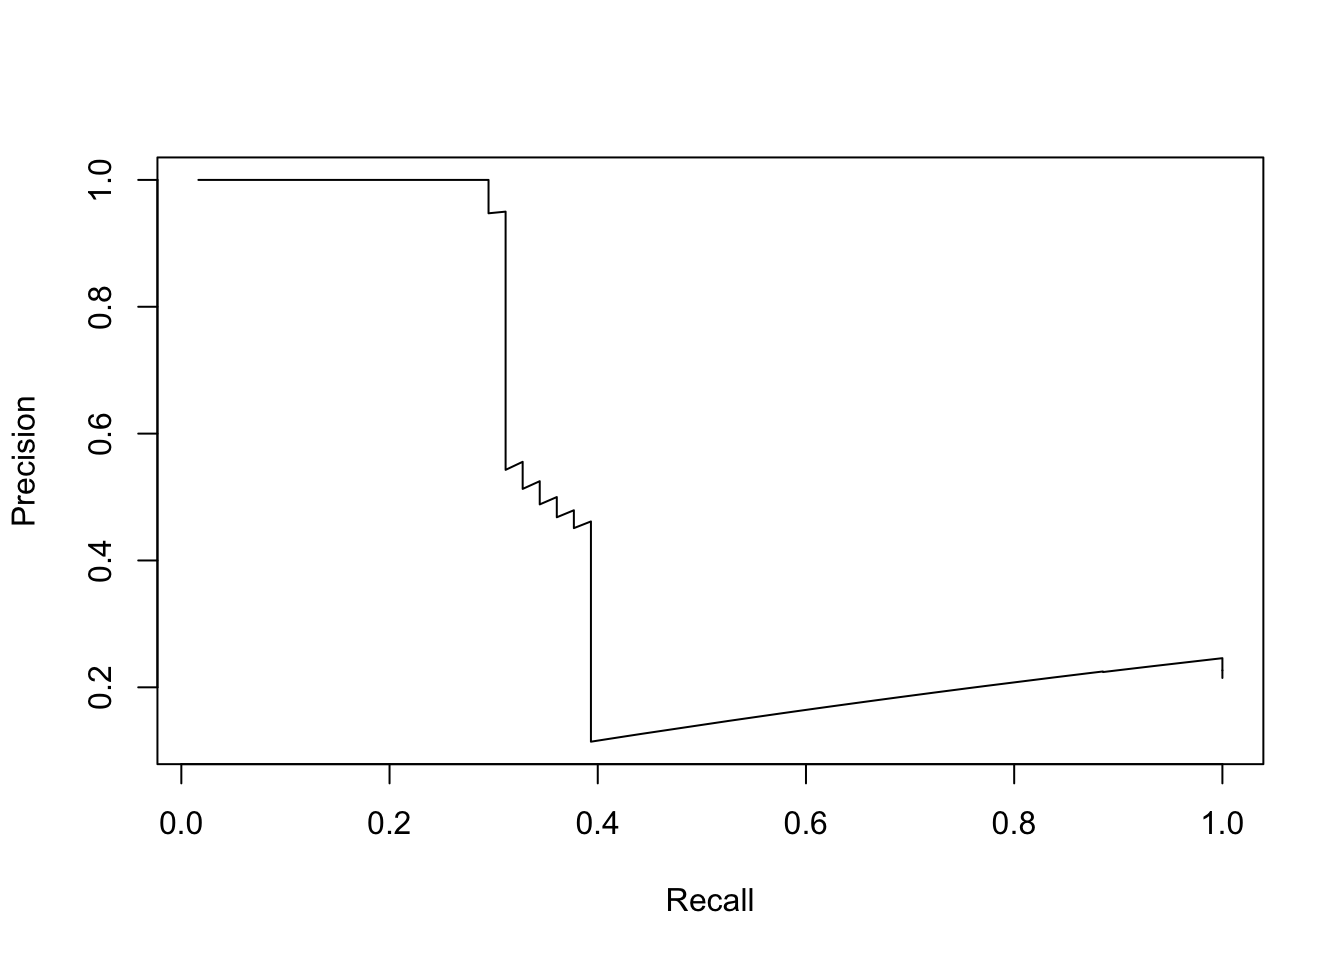
\includegraphics[width=0.45\textwidth]{results/post-update/memleak/boost-samemodel-prc}
  }
  \subfigure[Receiver Operating Characteristic (ROC) Curve (AUC = 0.4854).]{
    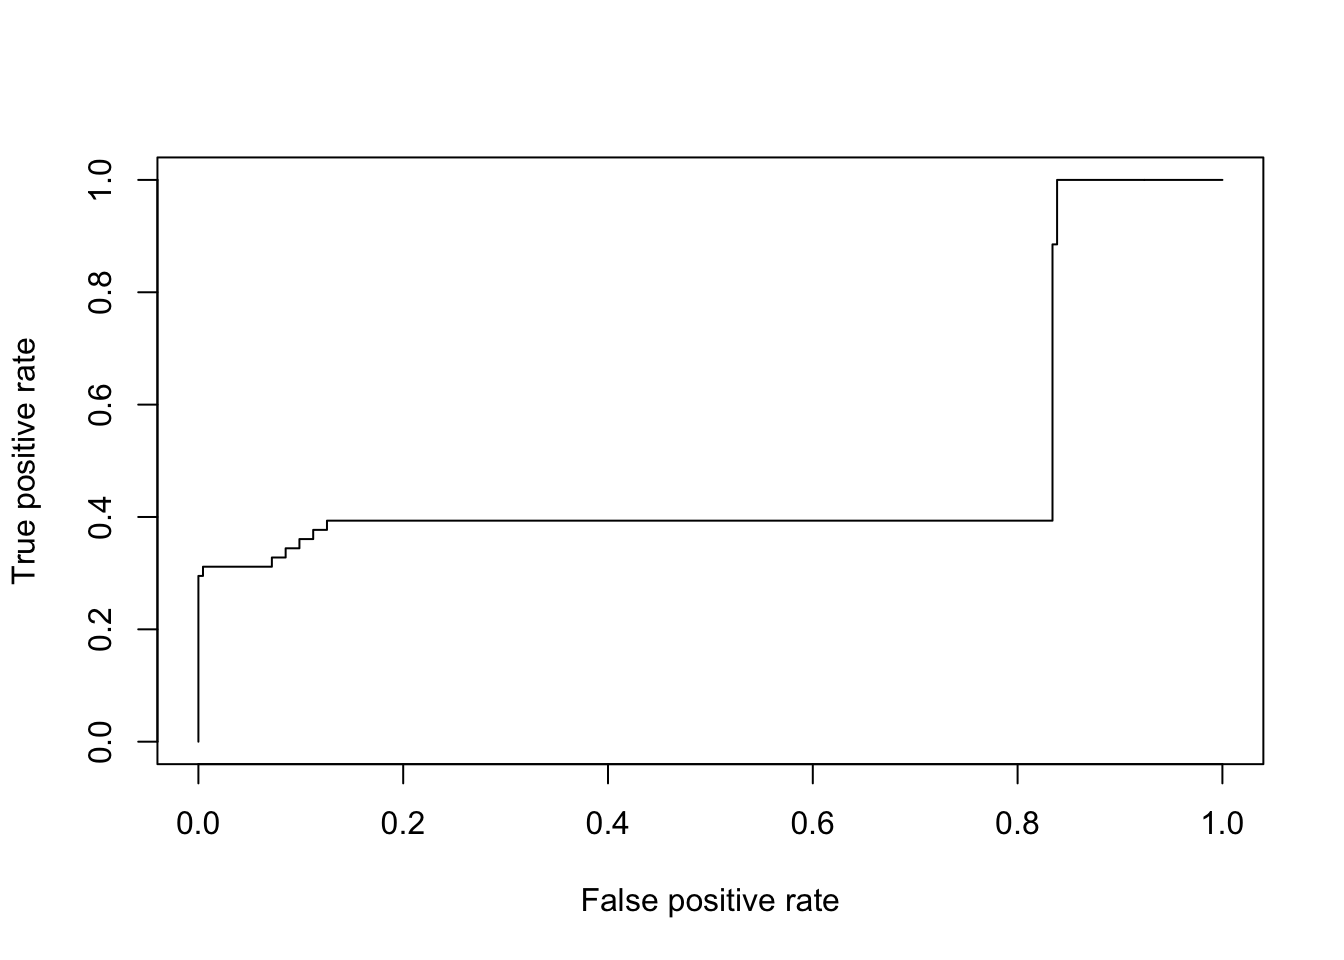
\includegraphics[width=0.45\textwidth]{results/post-update/memleak/boost-samemodel-roc}
  }
  \caption[Post-Update, Memory Leak Using Old Model Performance]{Performance of
  the boosting prediction method trained on failure data created before the
  software upate obtained by consuming all available memory until target
  application fails.}
  \label{fig:memLeakPostUpdateSameBoostedModel}
\end{figure*}
}

% Post-Update New Model
\newcommand{\figMemLeakPostUpdateBoostingPerf}{\begin{figure*}[ht!]
  \centering
  \subfigure[Precision/Recall Curve.]{
    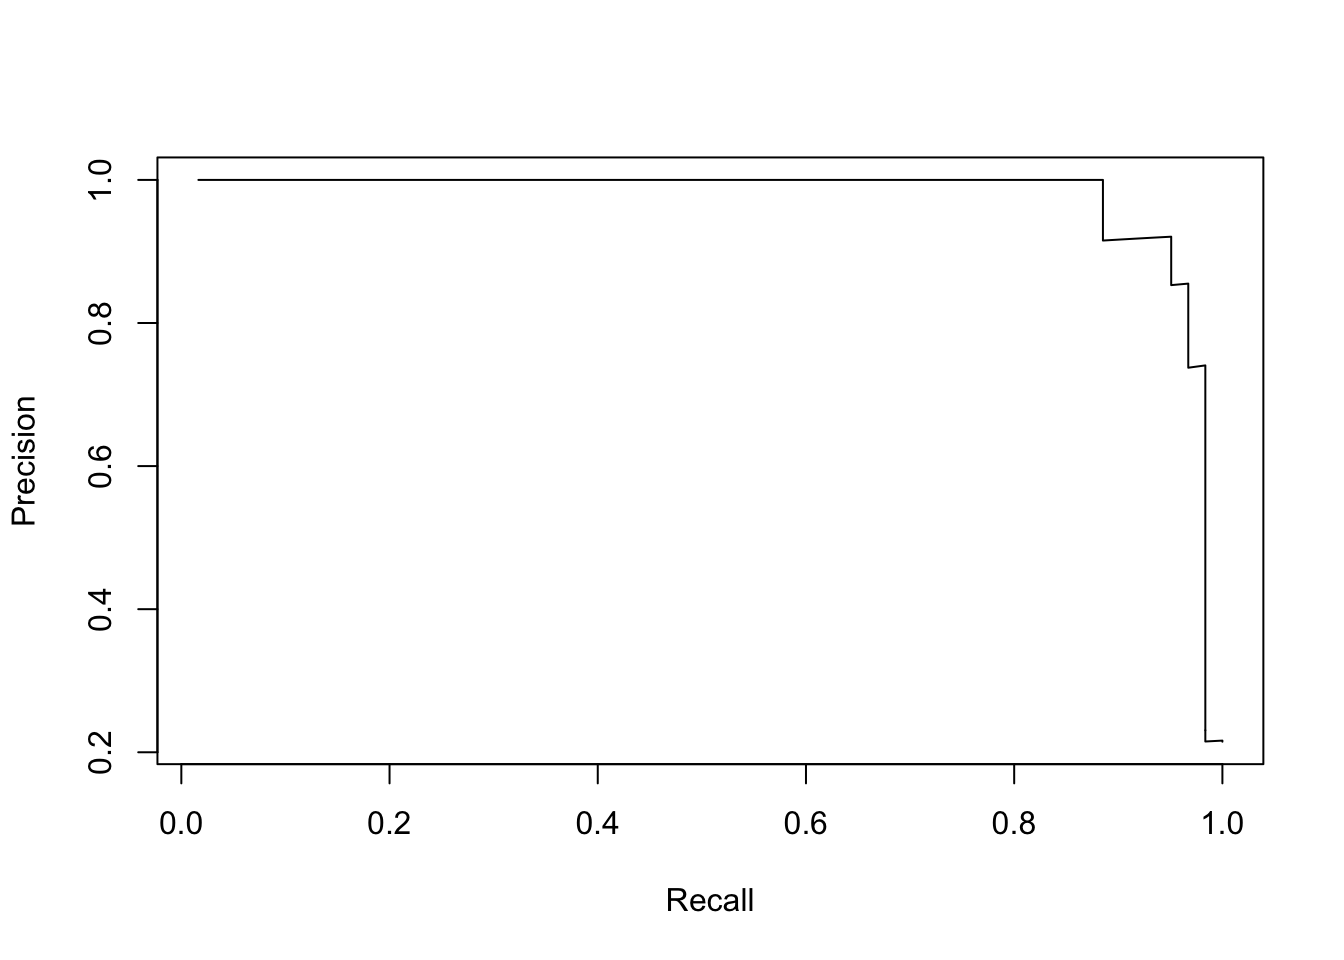
\includegraphics[width=0.45\textwidth]{results/post-update/memleak/boost-prc}
  }
  \subfigure[Receiver Operating Characteristic (ROC) Curve (AUC = 0.9801).]{
    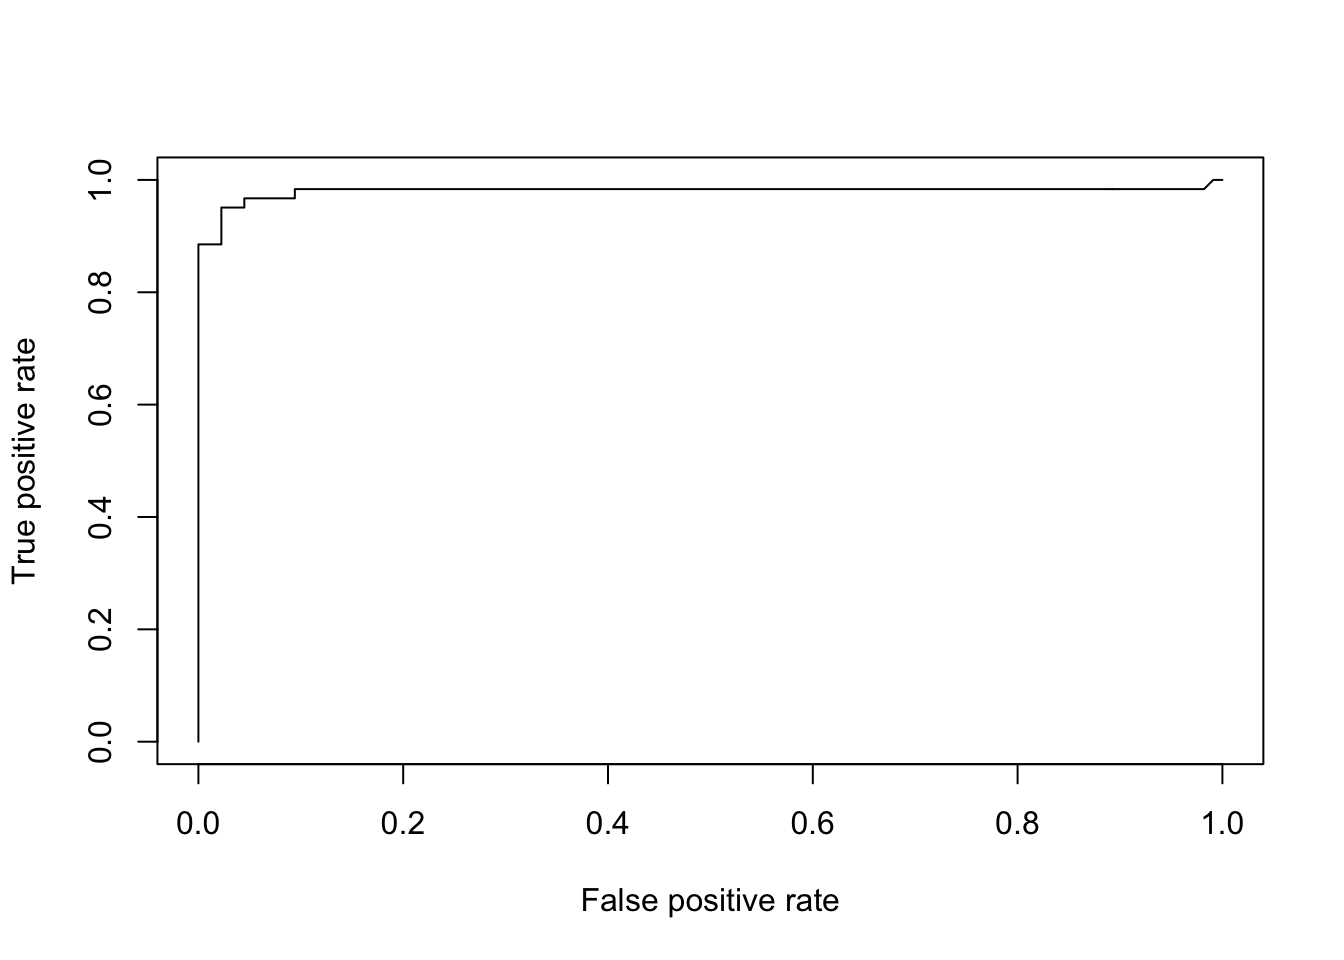
\includegraphics[width=0.45\textwidth]{results/post-update/memleak/boost-roc}
  }
  \caption[Post-Update, Memory Leak Using New Model Performance]{Performance of
  the boosting prediction method trained on failure data created after the
  software upate obtained by consuming all available memory until target
  application fails.}
  \label{fig:memLeakPostUpdateBoostingPerf}
\end{figure*}
}
